
\chapter{Introduction}

\label{chapter1}

Reinforcement Learning (RL) \citep{Sutton1998} is based on the idea of learning through experience, it is trial-and-error learning. A decision-making agent learns how to behave in an environment by interacting with it and receiving positive and negative reinforcement. This is akin to human and animal learning, and comes from the field of Psychology through the studies of operant conditioning \citep{nla.cat-vn2770732}, which have shown that human and animal behaviour can be shaped through positive and negative reinforcement. Experience can only be gained by trying new things, however it is often infeasible to try everything. Hence, there is a need for exploration, where the agent tries new things and learns the consequences of its actions. However, indefinitely exploring means that the experience gained is never exploited - this gives rise to the so-called \textit{exploration versus exploitation} trade-off.
\\Consider a human trying to navigate a maze, as in Figure \ref{fig:maze}. At the beginning, they know nothing, so they must choose some path to try. If they realise this path leads to a dead end, then they receive negative reinforcement, and they will learn from this experience that this path is not a good one to take. This process will continue until they reach the exit of the maze, where they might receive some positive reinforcement. To escape the maze, the human must try new things; they must explore the maze and discover where the dead ends are, and which paths seem promising, but they also need to exploit the knowledge that they have gained, and follow paths which seem promising.
\\Exploration is a very important topic in RL, as it necessitates learning. However, to effectively learn, exploration must be efficient in terms of learning time and cost \cite{Thrun-1992-15850}.
Exploration methods vary widely, from  using optimism, such as R-MAX and OIM, to instrinsic motivation, such as ICM \cite{DBLP:journals/corr/PathakAED17}, to Bayesian approaches, such as Bayesin Q-Learning \cite{10.5555/944919.944941}. However, in practice random exploration, such as $\epsilon$-greedy \cite{Watkins:1989, conf/nips/Sutton95}, is ubiquitous.
% Random exploration precludes efficiency, since non-optimal behaviour is continually evaluated, long after it has been realised to be non-optimal. Furthermore, randomness implies a lack of intelligence; an intelligent agent should not exhibit random behaviour.
\\Automated Planning (or just Planning) \cite{DBLP:books/aw/RN2020, Lav06} uses embedded knowledge of the environment, in the form of a model, to determine the optimal sequence of successive actions to fulfil a goal. However, planning relies on the model to accurately represent the environment; which cannot be guaranteed, due to approximations and abstractions, and therefore planning can be quite fragile. As an example, consider Figure \ref{fig:maze} again. Imagine that the human is given a map of the maze, but the shortest path out of the maze is shown blocked by some obstacle, if the human purely follows the map, they will never get out. A clear distinction between Planning and RL is that Planning relies on previously obtained knowledge, whereas RL relies on obtaining knowledge through experience.
\\Although Planning and RL take different approaches to decision making, they may be combined, which is known as Model-Based RL (MBRL). Most commonly MBRL is encapsulated in the form of planning over a learnt model, which has been shown to be very successful in recent years  \cite{silver2017mastering, pmlr-v28-levine13}. MBRL may also be used to guide and constrain exploration, such as DARLING \cite{AIJ16-leonetti}, UBE \cite{DBLP:journals/corr/abs-1709-05380} and MAX \cite{DBLP:journals/corr/abs-1810-12162}, resulting in faster, more efficient learning. Coming back to the example in Figure \ref{fig:maze}, the human could reason to try the blocked path, realise it is not actually blocked, and then update the map for the next person.
\\Within this work we explore the development of a framework that synergises planning and learning in order to drive and constrain exploration by making intelligent hypotheses about the environment, informed by the inherently inaccurate, but still useful, model, previous experience and environmental observations, rather than through randomness. The ultimate goal of this work is to mitigate the effect of the inherent inaccuracies in the model on the quality of learned behaviour; resulting in agents that can learn beyond the inaccuracies of the model, through intelligent exploration.

\begin{figure}[h!]
    \centering
    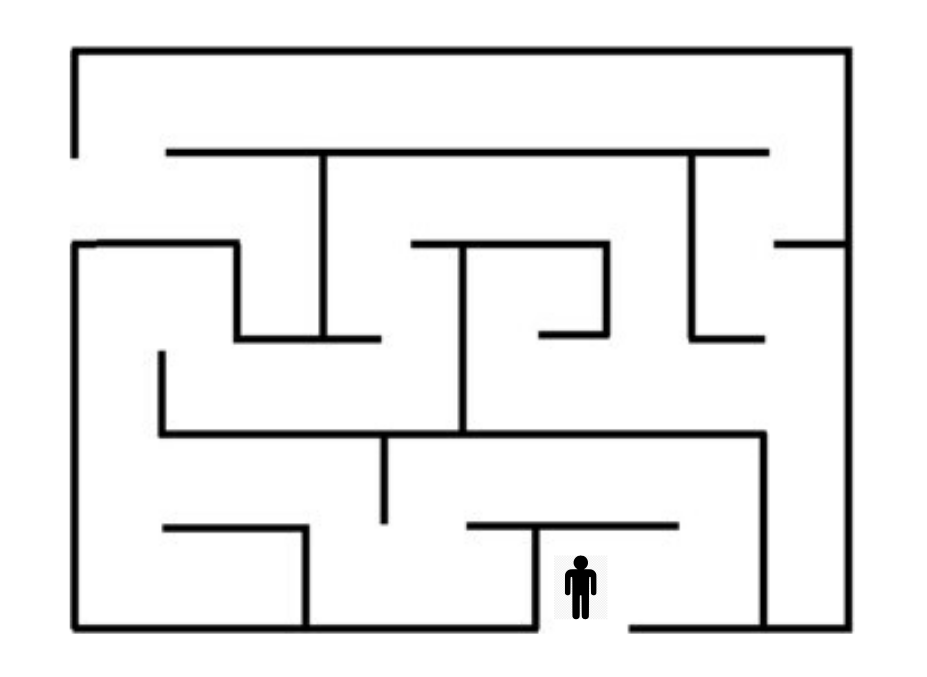
\includegraphics[max size={200}{200}]{report/assets/maze.png}
    \caption{Maze Navigation}
    \label{fig:maze}
\end{figure}